
\chapter{The experiment} % Main chapter title
\label{experiment}
During this thesis the ideas for the experiment changed a lot, we started by mimicking the architecture and features from Exposure to see if we could reproduce their experiment. We rapidly realized that their features were very complicated to obtain for almost all the datasets we could find. We also realized that we didn't have a continuous improvement of our classifier because we didn't have access to a live environment passive DNS capture as Bilge et al. did. That is when we realized a gap that we could try to fill. We decided to use the most pertinent aspects of Exposure's architecture and features and combine them with the research we did on all the current techniques used to abuse the DNS protocol.
\section{Pipeline of the research}
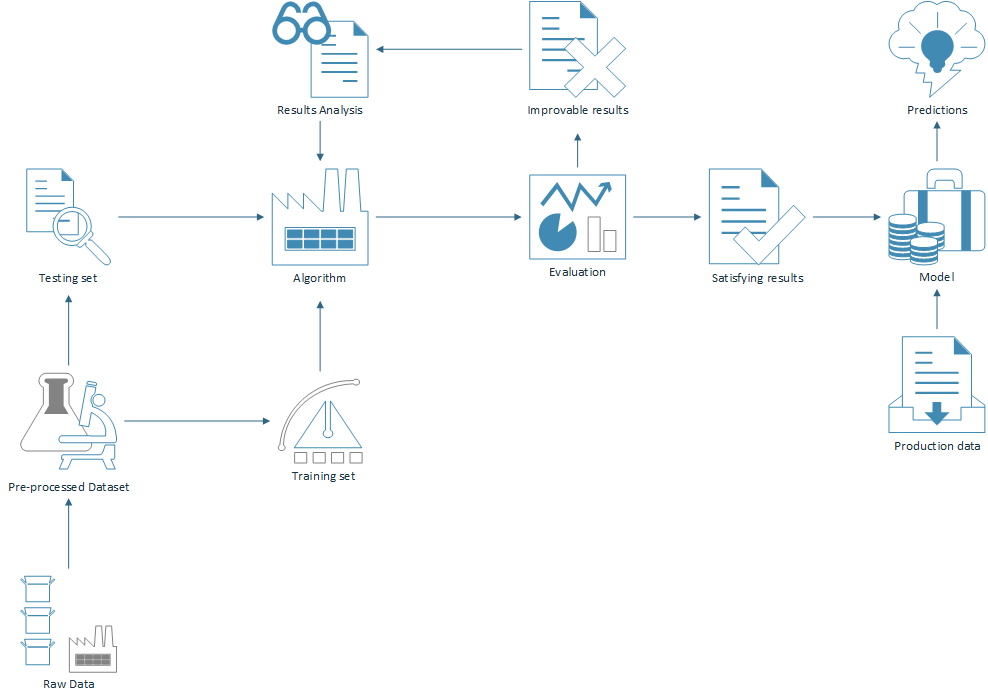
\includegraphics[scale=.6]{img/pers_ml_workflow.png}
The pipeline we created follows the machine learning workflow of a classification problem. We started by curating the dataset, transforming the captures into list of features, extracting and computing all the features studied. The next processing is the labeling. At this point, we have data that can be ingested by supervised algorithms. Before that, we do a first analysis of the features and go through the feature selection process. \\
During this feature selection we create a couple of different sets of features that will will use to train.
From there, we balance our dataset and we split it into 2 sets, the training set and the testing set. 
We train the classifiers with the different algorithms we have decided to use which are . During this training process, we use a feedback loop to change the features used and test out different hyper-parameter optimization techniques. We then test the predictions of our classifiers against the testing set. And finally, we analyze our results and draw some conclusions on our experiment.

 Extraction of the features and labeling.
Visual analysis of the distributions of the features and correlation
analysis. From there we assess the features through the classifiers in
specific cases. The general case with all the features, then depending
on the correlations found in the previous step we assess groups of features.
For the classification process, we have taken 5 classifiers that
have proven their potential to see if any has a better way to classify
the data. The classifiers used in the DGA analysis were Logistic regression,
linear discriminant analysis, k-nearest neighbors, decision
tree classifier and Naive Bayes. After training the classifiers, we test
the out by predicting the evaluation set with the best classifiers.
\section{Environment}

python 3
pandas
scikit-learn
numpy
jupyter
bro
pcap

https://norvig.com/ngrams/ (n-grams)

\section{Datasets}

Use inspiration from z-thesis 6.2 Assembling the Training Sets for the labeling


TODO: reformat the dataset section.

Since some of the implementations that we are going to compare have a blacklist step, we have done a large research on the blacklists available. At first we only focused on botnets domains and IPs, but then realized that bots can query their C2 but also try to access any malicious domain or IP, either to upload or download relevant data for the bot. Therefore, the final blacklist used is a very large combination of blacklists that go from domains linked to malware or C2 to domains linked to suspicious phishing/adware campaigns. One of the websites that really helped in this process is \url{https://firebog.net/}. All these lists have been combined into a big unique blacklist used in some of the approaches presented here.\\\\

The first idea was to use basics lists with an additional check with the virusTotal API but it is a very long process et the amount of lookups is limited therefore not a viable solution. Instead we researched the blacklists used by virusTotal and other DNSBL providers and have a very long static list instead.

%--------------------

% Explain the different datasets
Let us talk about the datasets used to train the different classifiers and algorithms used in the thesis.\\
This is going to be very dependent on the approach, for unsupervised algorithms, we are going to train them with clean traffic and see its reaction to malicious traffic. For classification algorithms we are going to go for model training for manual tagging of traffic that is either malicious or clean.
The idea will be to test the algorithms on parts of the sets but also try them on completely different traffic and compare the results.
\\

Depending on the algorithms the datasets aren't the same, for supervised approaches, there is a need of labelled data. For that we have searched for unique DNS traffic coming from Botnets combined with clean generic traffic. We create different combinations of traffic to improve our understanding of what works in what scenarios.\\


The datasets used in this thesis come from different sources that try to provide labelled data or precise data from botnets. These different sources are the CIS (Canadian institute of Security) that provide datasets created for the research related to security on traffic, specifically for machine learning techniques. They have labelled data from a lot of different sources and protocols. The one they provided me is focused on different types of botnets.
The ISOT Http Botnet dataset consists of 2 different datasets: malicious DNS traffic generated by multiple botnets and benign traffic generated by generic software. 

The ISOT Botnet dataset which consists in a large dataset regrouping 9 malicious botnets traffic in a controlled environment. 
And finally the CTU scenarios provided by the malware capture facility project.

SHOW SMALL TABLE WITH NUMBERS 

\section{Purpose of datasets}
The idea of having different datasets allows to understand if some techniques work against a large variety of evasion techniques or on specific ones. This also can be a way to propose complete feature set for complete detections.
\\
Finding proper datasets with botnet traffic with malicious DNS traces is not an easy thing to achieve. Luckily, the CIC team were kind enough to allow me to use their dataset designed for botnet traffic analysis. We also found a dataset proposed by the CTU which is a set of 13 scenarios that represent different types of malicious traffic generated by botnets. The CTU dataset was not as rich in DNS traffic as the other ones, but provided with fast flux traffic to test some of the features proposed to detect FF.

IMHERE
TODO: fill each of the sections for each dataset
\subsection{CIC}
Source\\
	Already mentioned
Content\\
	What are the botnets analyzed
Labeling\\
	How did we label them?
Use
	How did we use it in the study, we tested for example datasets for full training and testing, maybe we used certain datasets to train and others to test. Give more detail
This is a dataset maintained by the Canadian Institute for Cybersecurity. The have compiled malicious traffic from different sources and for most of them the traces are labelled which is very convenient for machine learning supervised approaches.\\ 
The dataset they provide for Botnet traffic analysis is composed of 9 different Botnets and of 2 datasets, a training and a testing dataset. Unfortunately, even being the largest labeled  dataset, the DNS traffic was low. 
\subsection{CTU}
Sources\\
	Already mentioned
Content\\
	What are the botnets analyzed
Labeling\\
	How did we label them?
Use
	How did we use it in the study, we tested for example datasets for full training and testing, maybe we used certain datasets to train and others to test. Give more detail
	
This is a set of datasets provided by the malware capture facility project\cite{CTU}. It captures malicious traffic from different malwares then provide them to the public for research. They also provide their own analysis on most of the datasets which provides insight on how the malware act and how it can be detected.\\
The scenarios that interest us are: the 5th and the 13th that include Fast-Flux labeled traffic.
It also provides hundreds of additional datasets but that are not as well documents and presented which makes the research for a particular dataset more complicated.
TODO: actually use all datasets to prove that we can detect any type of botnet traffic due to the general use of it.
\subsection{ISOT}
Sources\\
	Already mentioned
Content\\
	What are the botnets analyzed
Labeling\\
	How did we label them?
Use
	How did we use it in the study, we tested for example datasets for full training and testing, maybe we used certain datasets to train and others to test. Give more detail
	
This is a dataset specifically build around DNS traffic by the The ISOT Lab from the University of Victoria. It regroups 9 exploit kits ran in virtual environments in a closed network with a custom DNS server to snif all the traffic. This dataset provides us with 3 sets of traces, malicious, bening and a mix\cite{ISOT}.
	
\section{Dataset Processing}
Because of the amount of different features tested in the thesis. I decided to use 2 pcap extractors. The first was provided by our teacher Prof. J. Colin which is a very effective extractor and summarizes very well the relevant data for most of the features but for labeling and some of the features, more information was required. What we did to obtain a second extractor to complement the information was to run the traffic datasets through Bro, the network IDS. This provided us with DNS.logs, that we then converted using the python "bat" library which converts directly bro logs to dataframes.\\
Most of the labelled datasets actually only provided the IP addresses of the malicious traffic, this is why working with the bro logs was essential to label the datasets.
\subsection{cleaning}
\subsection{normalization}
\subsection{balancing the datasets}

\section{Assessment model (for features and models)}
provide information on how the results feedback are looped back into the algorithma

\subsection{Machine algorithms}
\subsection{Algorithm selection}
Based on the explanations above on how to chose the right algorithms, here we present the algorithms we will use. The reason for picking them is their mainstream use for this type of problem.

\subsubsection{Gaussian Naive Bayes}
This comes from the know probability and statistics Bayes' theorem. "It describes the probability of an event , based on prior knowledge of conditions that might be related to the event"\cite{bayes}. In ML learning the model saves the probabilities of each feature to belong to which category and when it is asked to predict new data, it does so by computing the event's probability to belong to each one of the categories. It bases its predictions on previous experience.

\subsubsection{K-Nearest Neighbors}
k-Nearest Neighbors (kNN) is a very simple supervised ML algorithm. kNN classifies new objects based on their nearest neighbors. The parameter k represents the amount of nearest neighbors it looks for before it assigns the majority. The model created by kNN is actually the entire training dataset since it will use all the neighbors to determine the classification of a new item. kNN algorithm works well with a low amount of features, with datasets with large dimensions computing the distances for the k-nearest neighbors becomes computationally expensive.

\subsubsection{Decision Trees}
Decision Trees(DTs) are supervised algorithms that based on observations of labeled data creates a model of decision that is represented by a tree where all the nodes of the tree are a condition for the features and where all the leaves are the label they are classified as. The classification process starts at the root and ends in one of the leaves.\\
DTs are very simple to visualize and perform really well even in higher dimensions. The most common problem of DTs is the overfitting of the data. Because outliers and unbalanced datasets will create branches that don't generalize the data correctly.

\subsubsection{Logistic Regression}
Logistic regression (LR) is a simple algorithm that is very effective in binary classification. Its core is the logistic function which transforms ranges of real-values into [0-1] ranges. What the logistic regression algorithm will do is through the use of weights of features, create the logistic function (model) for 1 of the classes and then for new values, it will output a probability which can be seen as a prediction of the input belonging to the class or not \cite{lr}.

\subsubsection{Support Vector Machine}
Support Vector Machine (SVM) is a supervised algorithm that excels in classification problems. The algorithm looks locally between the classes what hyper-plane separates them. 
Its hyper parameters are very interesting too, they allows to adapt to the dimension of the features to allow for transformations of the hyper-planes relative to the dimension. They also allow to tune how much we accept outliers. The tuning has to be done with care because we could end in an overfitting situation that doesn't generalizes enough and therefore could perform poorly with new data.

\subsubsection{XGBoost and Adaboost}
Both algorithms, eXtreme Gradient Boosting (XGBoost) and Adaptive Boosting (AdaBoost), are based on a similar concept which is boosting. Boosting is a technique that modifies weak learners into strong learners. It is done by training multiple of these weak learners sequentially and each improving based on the previous one.\cite{boosting} Both use this technique with different approaches to it.

\paragraph{AdaBoost}
The boosting used with Adaptive Boosting(AdaBoost) is simpler than XGBoost, it uses decision trees with a single decision node, they are called decision stumps. Each mistake made by stumps during classification are forwarded to the next stump by carrying more weight. This will allow the errors to be corrected of the numbers of stumps and obtain a cleaned up result in the end. This concept is mostly applied with DTs but it could be applied to any supervised algorithms. As are trees, AdaBoost are victims of outliers but they do a good job not to overfit the models as its peer. 

\paragraph{XGBoost}
The type of boosting used with XGBoost is Gradient Boosting on steroids. The algorithm improved is the RFs which is already a really strong supervised classifier. Like the AdaBoost, it sequentially improves the current tree using its predecessor but instead of adding more weight to the misclassified observations, it tries to train the next predictor to those observations. But this isn't all, XGBoost was created for fast and high performance to solve the slow characteristic of gradient boosting. That is where the eXtreme part comes in and where they introduced solutions to its shortcomings: parallelization of the tree construction,  distributed computing, out-of-core computing and cache optimization.\cite{xgboost} Due to this, it is one of the most popular algorithms because it provides the best performance on a range of difficult machine learning tasks. Its only drawback is its overfitting but that can be solved fine-tuning its hyper-parameters and it's explainability which can be complicated.

\subsubsection{Random forest}
The Random Forest (RF) algorithm is an improvement of the DTs. The concept is to randomly create low correlated models (forest) and give them the same input. It then picks the majority result as the prediction for the input. This technique provides a good way to protect from the overfitting that DTs are known for and to protect against individual errors of the trees. RF takes advantage of Bagging (Bootstrap aggregation) and Feature randomness to achieve this uncorrelated forest.
Bagging consists in giving all the trees the same amount of data but with replaced data (duplicates). Secondly feature randomness as its name implies, at each node the trees only take decision based on a subset of features.\cite{rf}

\subsubsection{Artificial Neural Networks}
Artificial Neural Networks (ANN) is an algorithm created similar to how the brain works and its learning capabilities by modeling neurons and their synapses. It works as a black box system with inputs on one side and and outputs on the other which are dependent on the inputs. The black box is a network of neurons grouped in layers, neurons of each layer connect with the ones of the next layer with weighted connections that will determine when the neurons fire. The modeling is around finding the values of the neurons and the connections inside the blackbox (hidden layers). The way ANNs hidden layers are computed are through gradient descent, a way of automatically updating the weights step by step into a direction that will make them less wrong, based on the output desired.\cite{ann}



\subsection{Feature extraction}
PCA

\subsection{Training and testing model}
We used 10-

\subsection{Results metrics}
TODO: remove this section
\cite{fitting}